\documentclass[sigconf]{acmart}

\usepackage{balance}
\usepackage{booktabs}
\usepackage{balance}

\setcopyright{rightsretained}
\acmDOI{10.475/123_4}
\acmISBN{123-4567-24-567/08/06}

\acmConference[12752]{Data Driven Building Energy Management}{Fall 2017}{CMU,
  USA}
\acmYear{2017}
\copyrightyear{2017}

\acmArticle{4}
\acmPrice{15.00}

\begin{document}
\title{Non-Intrusive Load Monitoring Using Occupancy Information and
  Ambient Information}
\titlenote{Fall 2017, 12752 Data Driven Building Energy Management
  Project}

\author{Pengji Zhang}
\affiliation{%
  \institution{Carnegie Mellon University}
  \streetaddress{5000 Forbes Avenue}
  \city{Pittsburgh}
  \state{Pennsylvania}
  \postcode{15213}
}
\email{pengjiz@andrew.cmu.edu}

\begin{abstract}
  Non-intrusive load monitoring is of great importance in smart
  infrastructures. This project attempts to incorporate prior
  knowledge about the residents into traditional Hidden Markov Models
  for non-event based appliance load monitoring. We build a model by
  utilizing the information on temperature and the locations of the
  residents to estimate the initial probabilities and transition
  matrices of an extended Hidden Markov Model dynamically. Our
  experiments of the model on one single appliance TV show that
  incorporating the prior knowledge of the residents could greatly
  improve the performance of conventional models.
\end{abstract}

\keywords{Non-intrusive Load Monitoring, Hidden Markov Model}

\maketitle

\section{Introduction}

Non-intrusive load monitoring (NILM) is aimed to estimate the
electricity consumption of each appliance from the aggregated
consumption, without installing any additional
sensors.~\cite{hart1992nonintrusive} Because of the rapid growth in
smart meter deployments all over the world---which provides an ideal
platform for collecting electricity consumption data and communicating
with consumers~\cite{kim2011unsupervised, parson2012non}---we can
expect NILM will be of great importance in the future for the
management of the power system.~\cite{kim2011unsupervised}

Many approaches have been proposed to solve the NILM problem. Even
though the methods of those solutions are very different from each
other, most of them relies heavily on the power load data to train the
model. For example, Parson et al.\@ used the aggregated power load
data to learn the transition matrix and the emission matrix for each
appliance in the setting of a hidden markov
model;~\cite{parson2012non} Hart et al.\@ used a model to detect and
attribute the significant changes in the power
load.~\cite{hart1992nonintrusive} However, given the rise of
\emph{smart cities} and \emph{internet of things}, we may have a lot
more information that can help us to improve the performance of
existing models. For example, the traffic flow information of a
certain day could tell us the times of people leaving or getting back
home, thus could tell us much information about the usage of
appliances. For another example, we may use the occupancy information
from the smart thermostat systems to better predict the usage of
certain appliances like TV, microwave, etc. Thus, for this project, we
would like to explore the feasibility of building a NILM solution with
\emph{not only the power load and the data for the power system, but
  also the ambient information and occupancy information.}

\section{DRED Data Set}

The data set we are going to use is the Dutch Residential Energy
Dataset (DRED).~\cite{uttama2015loced} The data set contains the
appliance level energy monitoring data, the ambient information
(indoor and outdoor temperatures, wind speed, humidity and
precipitation) and the room-level occupancy information of one
household, over a period of 6 months from 5th July to 5th December
2015.~\cite{uttama2015loced}

Figure~\ref{fig:dred} shows the layout of the household as well as the
locations of the appliances and the sensors.

\begin{figure}[ht]
  \centering
  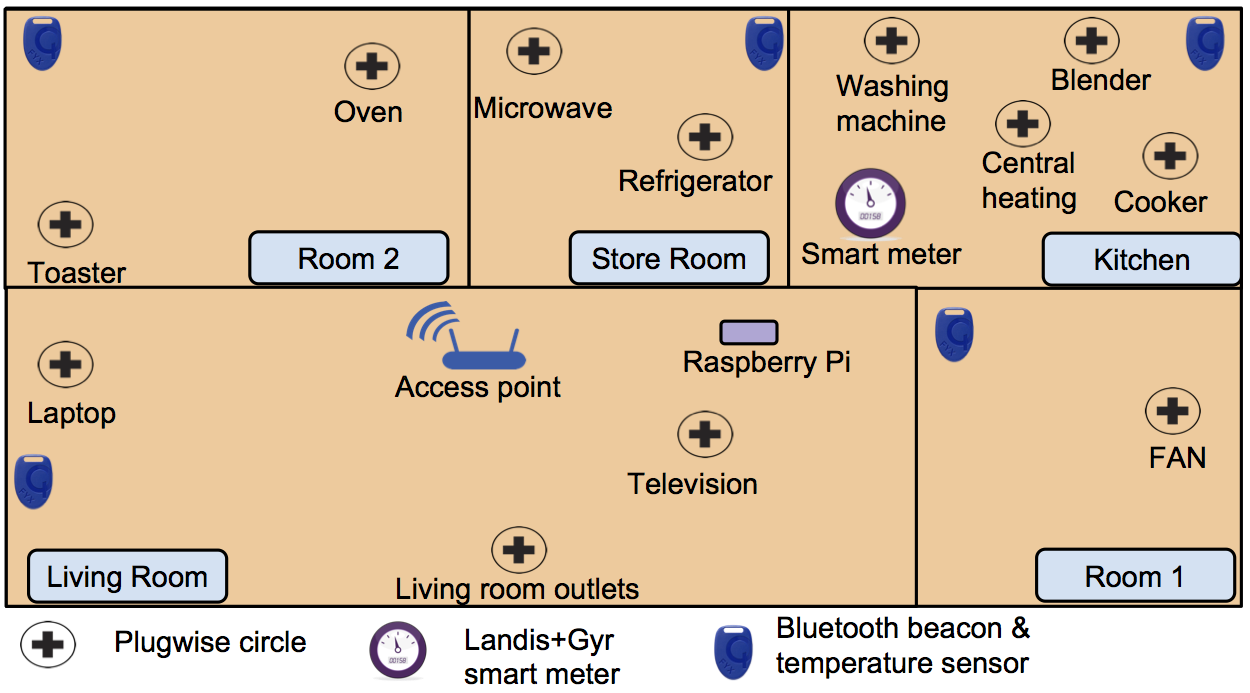
\includegraphics[width=0.45\textwidth]{figures/dred}
  \caption{\label{fig:dred} Household layout and the deployments of
    sensors in DRED.~\cite{uttama2015loced}}
\end{figure}

\section{Methods}

There are two parts in our model: softmax regression for estimating
the parameters of a hidden Markov model and an extended hidden Markov
model for predicting the states of appliances according to the total
power load of a household.

The whole process is shown in Figure~\ref{fig:methods}.

\begin{figure}[ht]
  \centering
  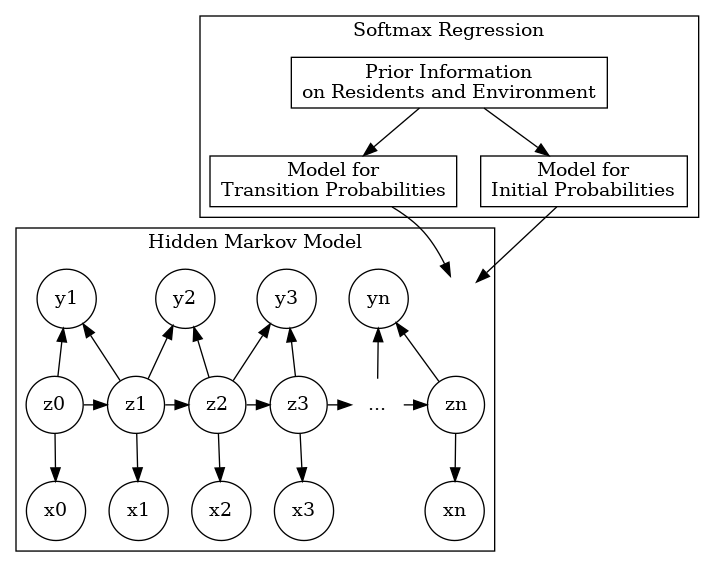
\includegraphics[width=0.45\textwidth]{figures/methods}
  \caption{\label{fig:methods} Methods for this project. Two softmax
    regression models are fitted to predict the parameters for an
    extended HMM model proposed by Parson et al.~\cite{parson2012non},
    which will be used for predicting the states of appliances from
    the total power demand of the household.}
\end{figure}

\subsection{Softmax Regression for Estimating Transition/Initial
  Probabilities}

Softmax regression is one of the multi-class version for conventional
logistic regression. It is capable to output the probabilities of each
class, which makes it a good choice for estimating the probabilities
in a hidden Markov model. The form of softmax regression model is
shown in Equation~\ref{eq:softmax}.~\cite{heckerman1997models}

\begin{equation}
P(y = k|\mathbf{x}; \theta) = \frac{\exp(\theta^{(k)T}\mathbf{x})}{\sum_{i~= 1}^{K}\exp(\theta^{(i)T}\mathbf{x})}
\label{eq:softmax}
\end{equation}

The features we will use in the model for initial probabilities include
\begin{enumerate}
\item Temperatures at different locations as shown in
  Figure~\ref{fig:dred}.
\item Occupancy information of each room. For this feature, we use the
  percentage of the residents being detected in one room out of total
  number of records in one minute. For example,
  \begin{equation}
    O_{\text{kitchen}}^{k} = \frac{\text{Number of records in kitchen in the
      } k\text{th minute}}{\text{Total number of records in the } k\text{th
        minute}}
    \label{eq:occupancy}
  \end{equation}
\item Hour of the day. This feature is to capture the daily patterns
  of appliance usage.
\item Day of the week. This feature is to capture the weekly patterns
  of appliance usage.
\end{enumerate}

Note that in this project the last two features are encoded with
one-hot-encoder.

\subsection{Extended Viterbi Algorithm for Decoding the States of
  Appliances}

The algorithm we choose to predict the states of one appliance from
the total energy consumption is an extended Viterbi algorithm based on
the work of Parson et al.~\cite{parson2012non} Parson et al.\@
proposed an extended Viterbi algorithm for decoding the hidden states
in the hidden Markov model shown in Figure~\ref{fig:hmm}.

\begin{figure}[ht]
  \centering
  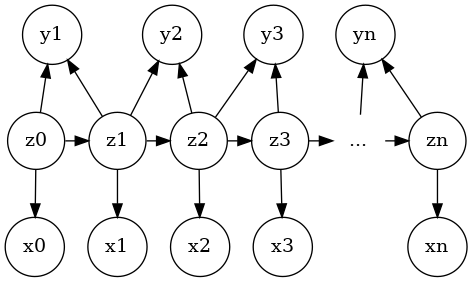
\includegraphics[width=0.45\textwidth]{figures/hmm}
  \caption{\label{fig:hmm} The hidden Markov model with two observed
    variables $x$ and $y$.}
\end{figure}

In their model,
\begin{align}
  \begin{split}
  p(\mathbf{x}, \mathbf{y}, \mathbf{z}|\mathbf{\theta}) &=
                                                          p(z_{1}|\mathbf{\pi})\prod_{t=2}^{T}p(z_{t}|z_{t-1},\mathbf{A})\\
                                                        &\prod_{t=1}^{T}p(w_{z_{t}} \leq x_{t}|z_{t}, \phi)\prod_{t\in
                                                          S}f(y_{t}|z_{t}, z_{t-1}, \phi),
  \end{split}
\end{align}
where
\begin{align}
p(w_{z_{t}} \leq x_{t} | z_{t}, \phi) &= \frac{1}{2}\left[ 1 +
  \mathrm{erf}\left( \frac{x_{t} -
  \mu_{z_{t}}}{\sigma_{z_{t}}\sqrt{2}} \right) \right] \\
f(y_{t} | z_{t}, z_{t-1}, \phi) &=
  \frac{1}{\sqrt{2\pi\sigma^{2}}}\exp\left( -\frac{y_{t} - (\mu_{z_{t}}
  - \mu_{z_{t-1}})}{2\sigma^{2}} \right).
\end{align}

We further extend this model by injecting information of occupancy and
environment in the transition probabilities and initial probabilities,
\begin{align}
  \mathbf{\pi} &= \mathrm{g}(I_{1}) \\
  \mathbf{A_{t}} &= \mathrm{g'}(I_{t}),
\end{align}
where $\mathrm{g}$ and $\mathrm{g'}$ are the two models from the
softmax regression on the training samples. Our algorithm does not
assume one single parameter for the whole hidden Markov model, instead
the parameters change with time according to the external information.
We suppose this would improve the performance because it captures more
variation in the process.

Besides, we will also use moving window smoothing to smooth the
predicted state sequences.

\section{Results}

\subsection{Data Preprocessing}

In the DRED data set, the minimum sampling frequency in the data set
is 1 Hz for the temperature data, so in the experiment, we choose to
take the mean values within each minute of all the variables to align
the sampling frequencies.

The records of the appliance `TV' are used to evaluate our model. This
data set contains the power demand of each appliance, but does not
contain the states. Therefore, we set the states as `off' when the
power demand is near zero, and `on' otherwise (See
Figure~\ref{fig:tv-power}). This is not a very precise way for this.
We may use some automated process with the current and voltage data to
better classify the states. However, this manual way should be enough
for testing our model in this project.

\begin{figure}[ht]
  \centering
  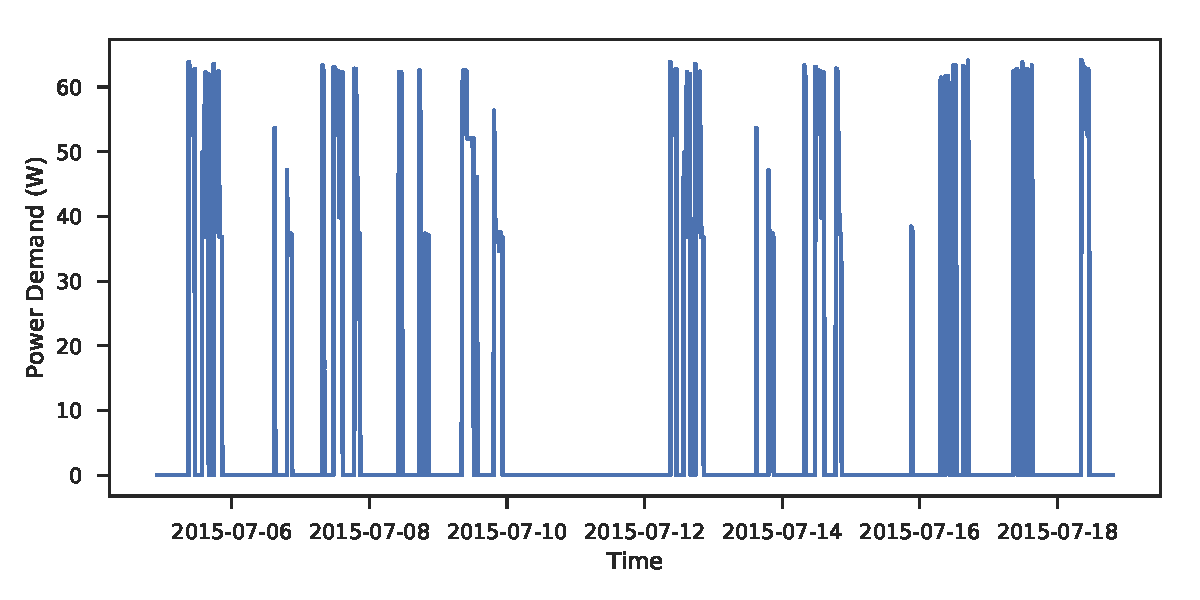
\includegraphics[width=0.45\textwidth]{figures/tv_power}
  \caption{\label{fig:tv-power} Mean power demand of TV in one minute.}
\end{figure}


Then we need to split the data set into two parts: one for the softmax
models and the other one for the HMM.\@ Because there are many gaps in
the data set (Figure~\ref{fig:gaps}) and large gaps will greatly
influence the performance of hidden Markov models but not the
performance of softmax regression models, which do not rely on time,
so we choose a range of samples that has small gaps for the HMM
model and other samples for the softmax models.

\begin{figure}[ht]
  \centering
  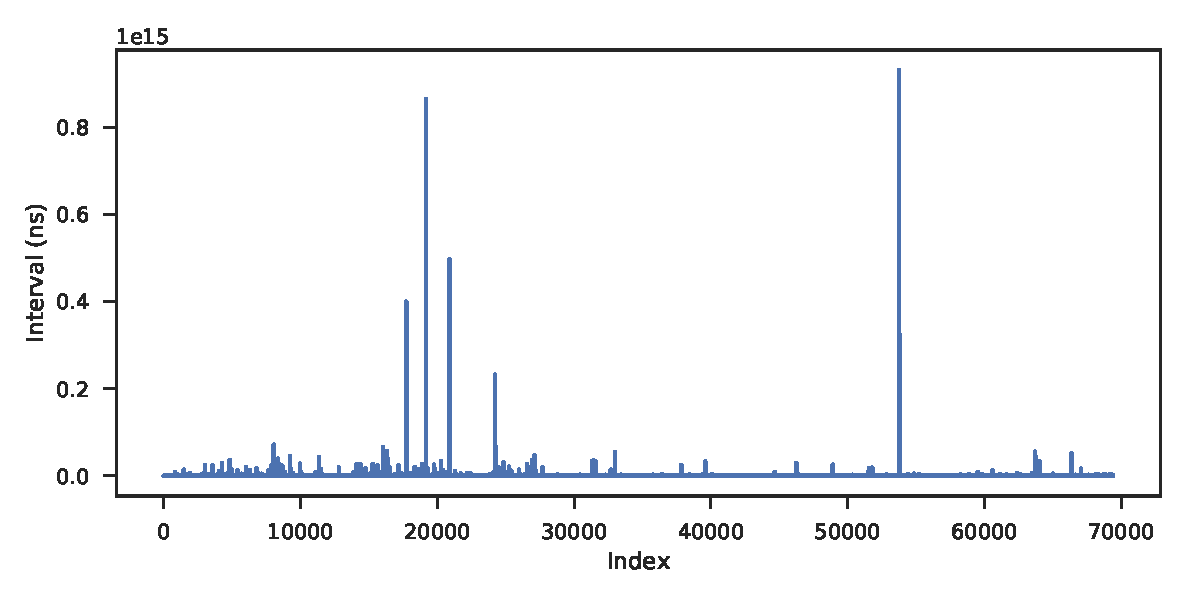
\includegraphics[width=0.45\textwidth]{figures/gaps}
  \caption{\label{fig:gaps} Intervals between consecutive samples (in
    nano seconds). The 42,000th to 47,000th samples are used in the HMM,
    other samples are used to fit the softmax models.}
\end{figure}

\subsection{Softmax Regression}

In our experiment, we pick a few models with different regularizers
and strengths of regularization. Figure~\ref{fig:softmax-metrics}
shows the results of 5-fold crossing validation of those models and
the performance of the baseline model (one single set of probabilities
obtained by counting).

\begin{figure}[ht]
  \centering
  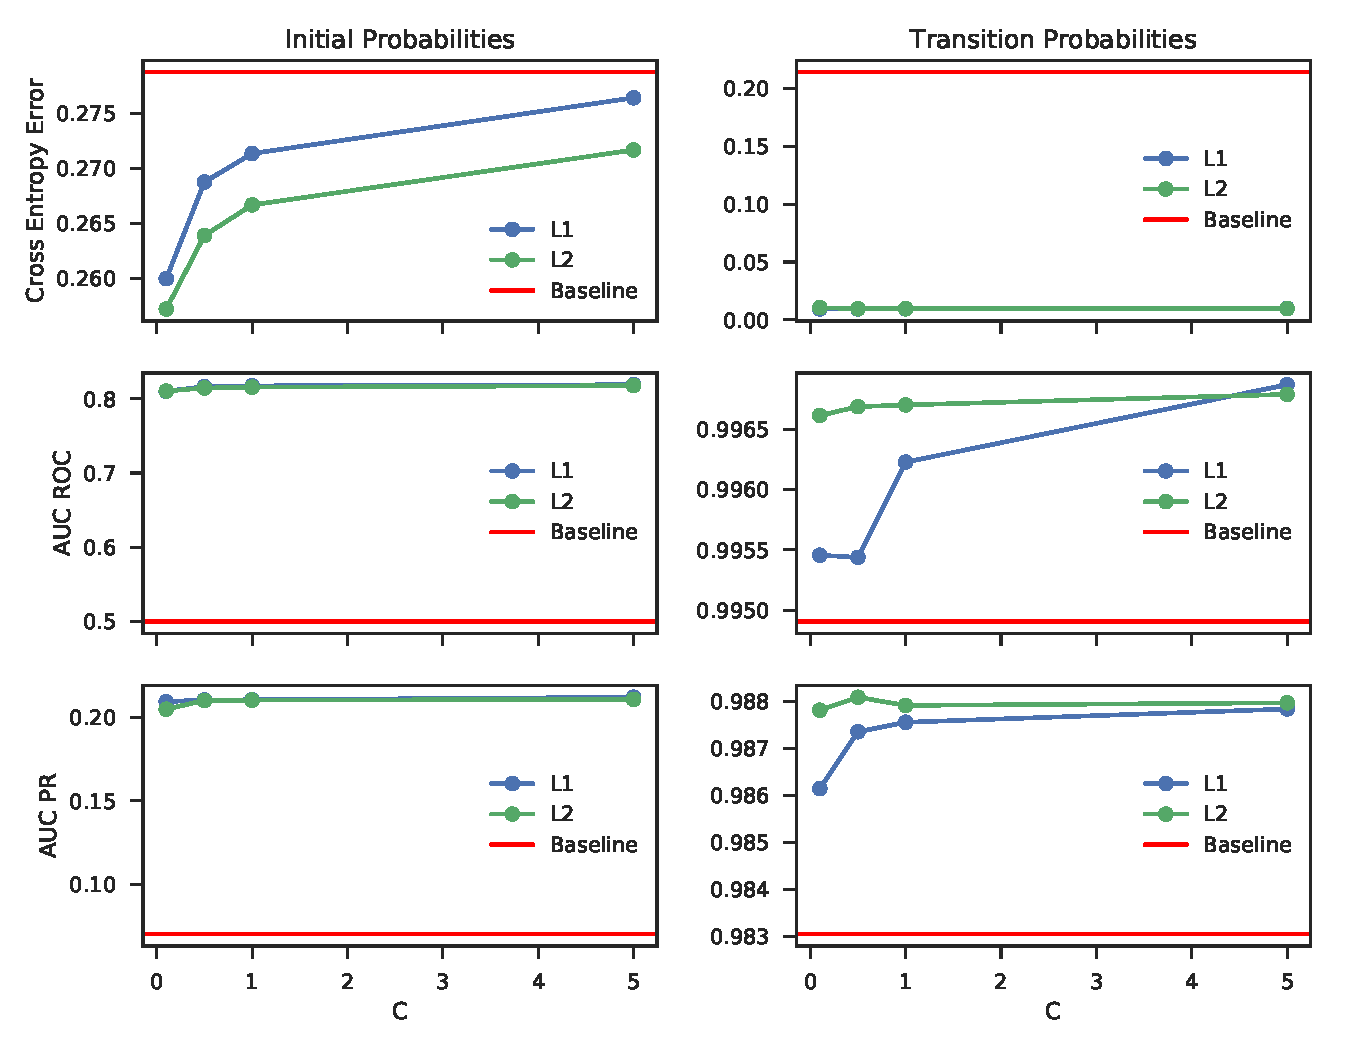
\includegraphics[width=0.45\textwidth]{figures/softmax-metrics}
  \caption{\label{fig:softmax-metrics} Cross entropy losses, AUC ROC
    and AUC PR of different models.}
\end{figure}

We can see that the models do improve the accuracy of estimating the
probabilities, even though for predicting initial probabilities those
models are not very ideal---the AUC of the PR curve is about 0.2 only.

We know that by nature the usage data of many appliances are
imbalanced---many appliances are at the `off' state most of the time,
like the toaster, while some other appliances are at the `on' state
most of the time, like the fridge. So we choose the model with good
AUC ROC as well as AUC PR scores as our final model, i.e.\ the model
with L2 regularizer and $\lambda = \frac{1}{C} = 1$.

\subsection{Decoding the States}

With the fitted model, we will use the extended Viterbi algorithm to
predict the states of the appliance of interest---TV.\@ The window
size of the smoother is 3, and the threshold for accepting
$f(y|z_{t}, z_{t - 1})$ as defined by Parson et
al.~\cite{parson2012non} is 0.033. Figure~\ref{fig:hmm-results} shows
the results.

\begin{figure}[ht]
  \centering
  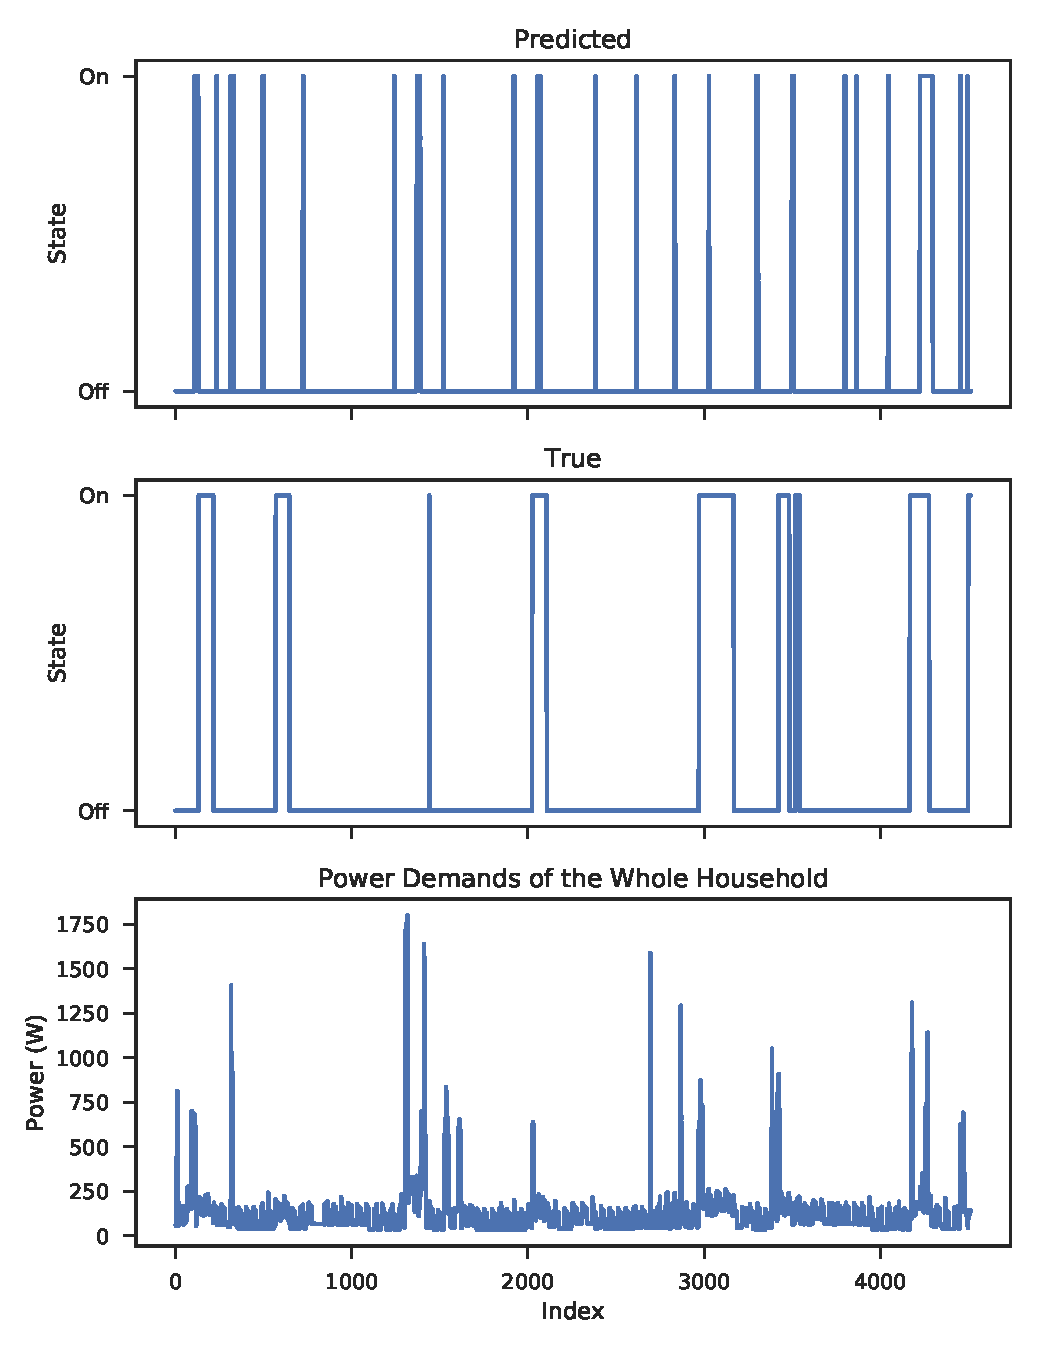
\includegraphics[width=0.45\textwidth]{figures/hmm-results}
  \caption{\label{fig:hmm-results} Predicted states, true states and
    power demands of the household.}
\end{figure}

We can see that the predicted sequence is more unstable compared to
the true values.

Figure~\ref{fig:cm} shows the confusion matrix. There are a lot of
false `off' states. The F1 score of the model is only 0.14, which is
not very satisfying.

\begin{figure}[ht]
  \centering
  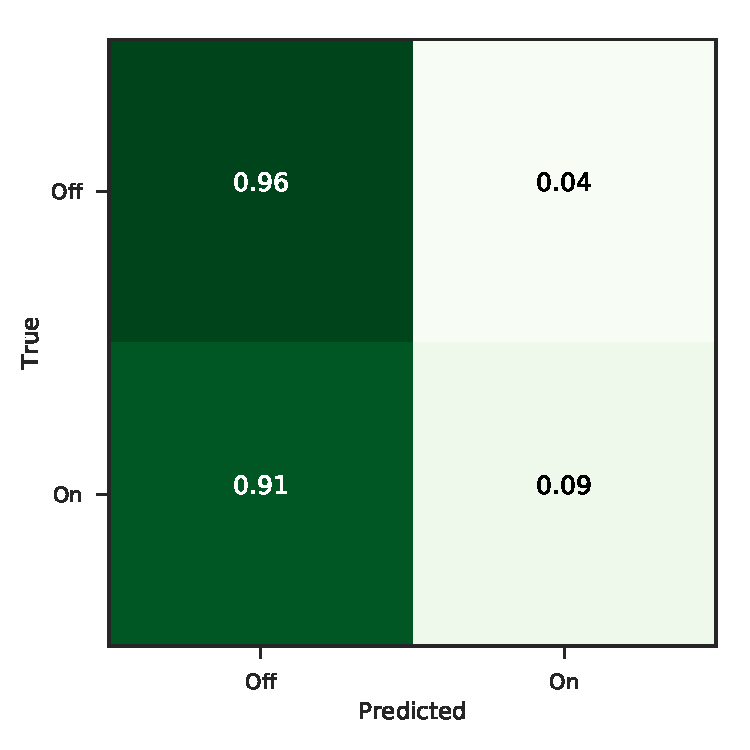
\includegraphics[width=0.3\textwidth]{figures/cm}
  \caption{\label{fig:cm} Normalized confusion matrix of the model on
    the test set.}
\end{figure}

\balance{}

\section{Discussion}

With a hidden Markov model, injecting information of the residents and
the environment will help improve the accuracy of the parameters, but
the performance of the whole model on non-intrusive appliance load
monitoring tasks is still not very impressive. We suppose this is
because the noise from other appliances. In the hidden Markov model
with two observed variable structure, much information on the state
change of the appliance comes from the variable $y$, which is the
differences between two consecutive power demands of the whole
household. However, some appliances like fridges may interfere the
prediction process of the model. From Figure~\ref{fig:hmm-results} we
can see that when the television is at the `On' or `Off' state, the
power demand of the whole house is still changing, which may make the
model to produce false state changes.

For the future work, we will bundle certain appliances as a group, and
predict their states with the factorial hidden Markov model. We think
this will help avoid the `dancing' of predictions but will not
require as much computation as the full factorial hidden Markov model
that includes all the appliances.

We may also try to collect more data on the residents and environment,
such as the age, number of residents in the house, etc. We think such
information will further improve the accuracy of our model.

\bibliographystyle{ACM-Reference-Format}
\bibliography{references.bib}

\end{document}


%%% Local Variables:
%%% mode: latex
%%% TeX-master: t
%%% End:
